\documentclass[11pt]{article}
\usepackage{header}
\def\title{HW 03}

\begin{document}
\maketitle
\fontsize{12}{15}\selectfont

\begin{center}
    Due: Saturday, 9/17, 4:00 PM \\
    Grace period until Saturday, 9/17, 6:00 PM \\
\end{center}

\section*{Sundry}
Before you start writing your final homework submission, state briefly how you worked on it.  Who else did you work with?  List names and email addresses.  (In case of homework party, you can just describe the group.)

{\color{blue}{I worked with the following members to complete this homework:

\begin{itemize}
    \item \textbf{Karena Chen (karena\_chen@berkeley.edu)}
\end{itemize}
}}

% {\color{blue}{I worked with \textbf{Emily Xiao emilyxiao@berkeley.edu} and \textbf{Karina Chen karena_chen@berkeley.edu}}}
\vspace{15pt}

\Question{Build-Up Error?}

What is wrong with the following "proof"? In addition to finding a counterexample, you should explain what is fundamentally wrong with this approach, and why it demonstrates the danger of build-up error.

\textbf{False Claim:}~If every vertex in an undirected graph has degree at least 1, then the graph is connected.

\begin{proof}[Proof?]
  We use induction on the number of vertices $n \ge 1$.

\emph{Base case:} There is only one graph with a single vertex and it has degree 0. Therefore, the base case is vacuously true, since the if-part is false.

\emph{Inductive hypothesis:} Assume the claim is true for some $n \ge 1$.

\emph{Inductive step:} We prove the claim is also true for $n+1$. Consider an undirected graph on $n$ vertices in which every vertex has degree at least 1. By the inductive hypothesis, this graph is connected. Now add one more vertex $x$ to obtain a graph on $(n + 1)$ vertices, as shown below.
\begin{center}
  \begin{tikzpicture}[node distance=0pt]
    \node at (1.5, 3.5) {$n$-vertex graph};
    \draw[dotted] plot[smooth cycle] coordinates {(0, 0) (0.5, 3) (2.5, 2.5) (2, 0)};
    \node[circ] (z) at (1.5, 2.5) {};
    \node[right=of z] {$z$};
    \node[circ] (y) at (1, 0.5) {};
    \node[below=of y] {$y$};
    \draw[dashed] plot[smooth,tension=0.9] coordinates {(z) (1, 2) (1.5, 1) (y)};
    \node[circ] (x) at (-1, 1) {};
    \node[above=of x] {$x$};
    \draw (x) -- (y);
  \end{tikzpicture}
\end{center}
All that remains is to check that there is a path from $x$ to every other vertex $z$. Since $x$
has degree at least 1, there is an edge from $x$ to some other vertex; call it $y$. Thus, we
can obtain a path from $x$ to $z$ by adjoining the edge $\{x,y\}$ to the path from $y$ to $z$. This
proves the claim for $n+1$. 
\end{proof}

\begin{solution}
    Clearly, we can construct an undirected graph with two cycles, in which the cycles are not connected to one another. Suppose we have 4 points:
    

    \begin{center}
        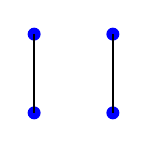
\begin{tikzpicture}
            \filldraw[blue] (0,0) circle (0.075cm);
            \filldraw[blue] (1, 0) circle (0.075cm);
            \filldraw[blue] (0, 1) circle (0.075cm);
            \filldraw[blue] (1, 1) circle (0.075cm);
            \draw[thick] (0,0) -- (0, 1);
            \draw[thick] (1, 0) -- (1, 1);
        \end{tikzpicture}
    \end{center}

    Each vertex in this graph has at degree at least 1, but clearly this graph is connected, and thus it is a direct counterexample. Now let's take a look at why this proof by induction does not work.

    The fundamental reason this proof fails is becuase our inductive step assumes that we build up the graph by inserting vertices in one by one, and connecting them to the main graph at each step. However, this does not have to be the case, and thus we arrive at a false conclusion.

    Another way to think about this is the fact that we are effectively \textit{forcing} the solution to be true by connecting each added vertex at every step, but this is not the only way to build a graph of $n+1$ vertices from $n$, thus leading to a logical fallacy.


  
\end{solution}
\pagebreak
\Question {Tournament}  

A \emph{tournament} is defined to be a directed graph such that for every pair
of distinct nodes $v$ and $w$, exactly one of $(v,w)$ and $(w,v)$ is an edge
(representing which player beat the other in a round-robin tournament).

Prove that every tournament has a Hamiltonian path. In other words, you can always
arrange the players in a line so that each player beats the next player in the
line.

\begin{solution}
    We prove this by induction. First, we specify that if player $a$ wins against player $b$, then we draw a directed arrow going from $b$ to $a$. We also assume no ties, since each vertex must be directed.

    \textbf{Base case:} $n = 2$. In a case with 2 people, one player wins against the other, so our Hamiltonian path is simply to start at the loser and walk along the edge towards the winner. 

    \begin{center}
        \begin{tikzpicture}
            \filldraw[blue] (0,0) circle (0.075cm) node[anchor=east, xshift=-0.25cm] {Player $A$};
            \filldraw[blue] (2,0) circle (0.075cm) node[anchor=west, xshift=0.25cm] {Player $B$};
            \draw[thick, -{Latex[scale=1.2]}] (2,0) -- (0,0);
        \end{tikzpicture}
    \end{center}

    So in this diagram, we assume without loss of generality that player $A$ won against player $B$, so our Hamiltonian path would be to walk from player $B$ to player $A$.

    \textbf{Inductive Hypothesis:} Assume that for a tournament of $n \geq 1$ people, that there exists a Hamiltonian path. Let's label the players $\{p_1, p_2, \dots, p_n\}$.

    Now we add a player to this group of $n$ people, call this player $P$. Notice that there are three possibilities: $P$ wins against everybody else, $P$ loses against everybody else, or $P$ wins some portion of their games. 

    If $P$ wins all their games, then it means that all vertices connected to $P$ point towards $P$. Thus, to draw our Hamiltonian path, we simply start at any player $p_i$ and end on another player $p_j$, then walk along the path from $p_j \to P$, which is guaranteed to exist since $P$ won all their games.

    If $P$ loses all their games, then it means that all vertices connected to $P$ point \textit{away} from $P$. To draw our Hamltonian path, we start at $P$ and walk along one of the edges to a player $p_j$, and follow the Hamiltonian path for our original group of $n$ people. 

    If $P$ loses some portion of their games, the same process applies: start at $P$, then walk along one of the edges from $P \to p_i$, then walk along the  Hamiltonian path of the original $n$ players. 

    Since in all cases there exists a Hamiltonian path, then we are done. $\blacksquare$.
\end{solution}
\pagebreak
\Question{Proofs in Graphs} 

\begin{Parts}

\Part On the axis from San Francisco traffic habits to Los Angeles traffic habits, Old California is more towards San Francisco: that is, civilized. In Old California, all roads were one way streets. Suppose Old California had 
$n$ cities ($n \geq 2$) such that for every pair of cities $X$ and $Y$,
either $X$ had a road to $Y$ or $Y$ had a road to $X$.

Prove that there existed a city which was reachable from every other city by traveling through at most 2 roads. 

[\textit{Hint:} Induction]

\begin{solution}
    We prove this by induction. 

    \textbf{Base case:} $n = 2$. If we have 2 cities, call them $X$ and $Y$. Then the road connecting the two either leads from $X \to Y$ or $Y \to X$. In either case, it's obvious that one of the two cities is reachable from the other by travelling through that road, and we are done. 


    \textbf{Inductive Hypothesis:} Assume that for $n$ cities, there exists one city that is reacahble from every other by travelling through at most 2 roads. We now prove that this is also the case for $n+1$ cities. 
    
    Suppose we have a graph of $n+1$ cities, and remove one node. Now, we have a graph of $n$ nodes, where there must exist one city (call it city $X$) that is reachable by travelling through at most 2 roads. 

    Now add the last city back, call this city $P$. Then, the connection of $P$ to $X$ can go in one of two directions. From $P \to X$ or from $X \to P$. If the connection is from $P \to X$, then we are done, since $X$ is reachable from $P$ using one road. 

    If the connection is from $X \to P$, look at the vertices that are 1 road away from $X$, and that point towards $X$. That is, these are the set of vertices $\{Y_1, \dots, Y_i\}$ such that they all have a road connecting $Y_i \to X$.
    
    If $X$ is reachable from 2 roads, then it follows that every $Y_i$ is reachable within 1 road. Now consider the roads connecting $Y_i$ and $P$. If the connection of one of these roads is $P \to Y_i$, then $X$ is reachable from $P$ within 2 roads. Otherwise, if all connections are $Y_i \to P$, then this means that every city is connected to $P$ within 2 roads, by travelling along the edge leading to $Y_i$ then travelling along $Y_i \to P$. Note that $X$ is also clearly connected to $P$ since the road between $X$ and $P$ is connected $X \to P$.
\end{solution}
\Part Consider a connected graph $G$ with $n$ vertices which has exactly $2m$ vertices of
odd degree, where $m > 0$. Prove that there are $m$ walks that \emph{together} 
cover all the edges of $G$ (i.e., each edge of $G$ occurs in exactly one of the $m$ walks, 
and each of the walks should not contain any particular edge more than once).

[\emph{Hint:} In lecture, we have shown that a connected undirected graph has an Eulerian tour if and only if every vertex has even degree. This fact may be useful in the proof.]

\begin{solution}
    We know that an Eulerian tour is simply an Eulerian walk which has the same starting and end point. Thus, we can construct our walks in the following method: 

    % Call the vertices with odd degree $\{X_1, X_2, \dots, X_{2m}\}$. Then, we pair a corresponding vertex $X_i$ with $X_j$, and a walk will consist of a path starting at $X_i$ and ending at $X_j$. Now we need to prove that these walks will guarantee that every edge is traversed.

    % Call the vertices with odd degree $\{X_1, X_2, \dots, X_{2m}\}$. Now mark all the vertices that are connected to each $X_i$ as the set $\{Y_1, Y_2, \dots, Y_i\}$
\end{solution}

\Part Prove that any graph $G$ is bipartite if and only if it has no tours of odd length.

[\emph{Hint:} In one of the directions, consider the lengths of paths starting from a given vertex.]
\end{Parts}
\pagebreak
\Question{Planarity and Graph Complements}

Let $G = (V, E)$ be an undirected graph.  We define the complement of $G$ as $\overline{G} = (V, \overline{E})$ where $\overline{E} = \{(i,j) \mid i,j \in V, i \neq j\} - E$; that is, $\overline{G}$ has the same set of vertices as $G$, but an edge $e$ exists is $\overline{G}$ if and only if it does not exist in $G$.

\begin{Parts}

\Part Suppose $G$ has $v$ vertices and $e$ edges.  How many edges does $\overline{G}$ have?


\begin{solution}
    There are ${v \choose 2} = \frac{v(v-1)}{2}$ possible edges in a graph of $n$ nodes. Thus, if $e$ of them are connected, then $\overline G$ will have $\frac{v(v-1)}{2} - e$ edges.
\end{solution}
\Part Prove that for any graph with at least 13 vertices, $G$ being planar implies that $\overline{G}$ is non-planar.

\begin{solution}
    In order for a graph to be planar, it must satisfy the relation:

    \[ e \leq 3v - 6\]

    So this must be true for a graph with larger than 13 vertices. If $G$ is planar, then it satisfies $e \leq 3(v - 2)$ so this means that $\overline G$ must have 

    \[ e' = \frac{v(v-1)}{2} - e\] 

    Now since $e$ is bouded above, then the minimum number of edges $\overline G$ must have is $\frac{v(v-1)}{2} - 3(v-2)$. To prove that $\overline G$ is not planar, we show the following inequality is true:

    \[ \frac{v(v-1)}{2} - 3(v-2) > 3(v-2) \implies \frac{v(v-1)}{2} > 6(v-2)\]

    for all $v \geq 13$. We can show this true by induction. 

    \textbf{Base case:} $v = 13$. We can verify this by plugging it in:

    \[\frac{13 \cdot 12}{2} = 78 > 66\]

    \textbf{Inductive Hypothesis:} Suppose this inequality holds for some $v \geq 13$. We show that this is also true for $v+1$. So we need to show:

    \[ \frac{v(v+1)}{2} > 6(v+1-2) = 6(v-1) \]

    Notice we can write the left hand side as 

    \[ \frac{v(v-1)}{2} + v > 6(v - 2) + v\] 

    Simultaneously, we can rewrite $6(v-1) = 6(v-2) + 6$, and since $v \geq 13 > 6$ then $6(v-2) + v > 6(v-1)$, and thus our inductive step is done. Therefore, our original statement is true, and we are done $\blacksquare$.




\end{solution}

\Part Now consider the converse of the previous part, i.e., for any graph $G$ with at least 13 vertices, if $\overline{G}$ is non-planar, then $G$ is planar. Construct a counterexample to show that the converse does not hold.

\textit{Hint: Recall that if a graph contains a copy of $K_5$, then it is non-planar. Can this fact be used to construct a counterexample?}

\end{Parts}
\pagebreak
\Question{Touring Hypercube} 

In the lecture, you have seen that if $G$ is a hypercube of dimension $n$, then
\begin{itemize}
    \item The vertices of $G$ are the binary strings of length $n$.
    \item $u$ and $v$ are connected by an edge if they differ in exactly one bit location.
\end{itemize}

A \emph{Hamiltonian tour} of a graph is a sequence of vertices
$v_0, v_1, \ldots, v_k$ such that:
\begin{itemize}
    \item Each vertex appears exactly once in the sequence.
    \item Each pair of consecutive vertices is connected by an edge.
    \item $v_0$ and $v_k$ are connected by an edge.
\end{itemize}

\begin{Parts}

    \Part Show that a hypercube has an Eulerian tour if and only if $n$ is even.
    

    \Part Show that every hypercube has a Hamiltonian tour. 

    

\end{Parts}
\pagebreak
\Question{Connectivity}

Consider the following claims regarding connectivity:
\begin{Parts}
    \Part  Prove: If $G$ is a graph with $n$ vertices such that for any two non-adjacent vertices $u$ and $v$, it holds that $\deg u + \deg v \ge n - 1$, then $G$ is connected. 
    
    [\textit{Hint:} Show something more specific: for any two non-adjacent vertices $u$ and $v$, there must be a vertex $w$ such that $u$ and $v$ are both adjacent to $w$.]

    \Part  Give an example to show that if the condition $\deg u + \deg v \ge n - 1$ is replaced with $\deg u + \deg v \ge n - 2$, then $G$ is not necessarily connected.

    \Part Prove: For a graph $G$ with $n$ vertices, if the degree of each vertex is at least $n/2$, then $G$ is connected. 

    % \begin{solution}
    %     We prove this by induction. 


    %     \textbf{Base case:} $n = 2$. In a connected graph with 2 nodes, there are $1 = 2/2$ vertices, proving the base case. 

    %     \textbf{Inductive Hypothesis:} Suppose that a graph with $n$ vertices with each vertex having degree $n/2$ is connected. 

    %     In a graph with $n+1$ vertices, it means that each vertex has at least $n/2 +1$ edges. Now we remove  
    % \end{solution}
    
    \Part Prove: If there are exactly two vertices with odd degrees in a graph, then they must be in the same connected component (meaning, there is a path connecting these two vertices). 
    
    [\textit{Hint:} Proof by contradiction.]

    \begin{solution}
        As per the hint, we prove this by contradiction. Suppose we have a graph with two odd vertices but they are not connected by a path. Call these vertices $V_1$ and $V_2$. Then it follows from this that there is no vertex connected to $V_1$ that connected to $V_2$, and vice versa. Thus, the graphs containing $V_1$ and $V_2$ can equivalently be thought of as separate graphs. 

        If they are separate graphs, then they must obey the property that $\sum_{v \in V} \deg v = 2|E|$. But since each graph only contains one node with an odd number of vertices, this sum cannot be odd, and thus we've arrived at a contradiction. Therefore, if there are exactly two vertices with odd degrees in a graph, then they must be in the same connected component. 
    \end{solution}
\end{Parts}
\pagebreak 
\Question{Edge Colorings}

An edge coloring of a graph is an assignment of colors to edges in a graph where any two edges incident to the same vertex have different colors. An example is shown on the left.

\begin{center}
    \begin{tikzpicture}
        \clip (-1, -1) rectangle (8, 2.1);

        \node[circ] (n1) at (0, 0) {};
        \node[circ] (n2) at (1, {sqrt(3)}) {};
        \node[circ] (n3) at (2, 0) {};
        \draw (n1) -- node[above left] {color 1} (n2)
        -- node[above right] {color 2} (n3)
        -- node[below] {color 3} (n1);

        \node[circ] (m1) at (5, 0) {};
        \node[circ] (m2) at (5, 2) {};
        \node[circ] (m3) at (7, 2) {};
        \node[circ] (m4) at (7, 0) {};
        \draw (m1) -- (m2) -- (m3) -- (m4) -- (m1);
        \draw (m2) -- (m4);
        \draw (m1) edge[out=-60, in=-30, looseness=2.5] (m3);
    \end{tikzpicture}
\end{center}

\begin{Parts}
\Part Show that the 4 vertex complete graph above can be 3 edge colored. (Use the numbers $1,2,3$ for colors. A figure is shown on the right.)

\begin{solution}
    We can colour the graph as follows: 

    \begin{center}
        \begin{tikzpicture}
            \node[circ] (m1) at (5, 0) {colour 1};
            \node[circ] (m2) at (5, 2) {};
            \node[circ] (m3) at (7, 2) {};
            \node[circ] (m4) at (7, 0) {};
            \draw (m1) -- (m2) -- (m3) -- (m4) -- (m1);
            \draw (m2) -- (m4);
            \draw (m1) edge[out=-60, in=-30, looseness=2.5] (m3);
        \end{tikzpicture}
    \end{center}
\end{solution}

\Part Prove that any graph with maximum degree $d \geq 1$ can be edge colored with $2d-1$ colors. 



\Part Show that a tree can be edge colored with $d$ colors where $d$ is the maximum degree of any vertex.


\begin{solution}
    If the maximum vertex has degree $d$, then it means that every other vertex has $\deg v \leq d$. If they are less than $d$, then 
\end{solution}

\end{Parts}

\end{document}
